\chapter{Grundlagen}
\label{ch:Grundlagen}

\todo[inline]{Schreiben der Einführung des Kapitels \ref{cha:grundlagen} Grundlagen}

\section{Verstärkendes Lernen(Reinforcement Learing)}
Beim bestärkenden Lernen ist der Lerner ein entscheidungstreffender Agent, der in einer Umgebung Handlungen ausführt und Belohnung (oder Bestrafung) für seine Aktionen beim Versuch, das Problem zu lösen, erfährt. Nach einer Menge an Versuch-und-Irrtum-Durchläufen sollte er die beste Vorgehensweise lernen, welche der Sequenz an Aktionen entspricht, durch welche die Gesamtbelohnung maximiert wird\cite[397]{Alpaydin}.

Ein Agent führt Entscheidungen (Aktionen) innerhalb einer ihm unbekannten Umgebung aus. Der Agent soll in dieser Umgebung ein Ziel erreichen. Dieses Ziel ist oftmals die einzige Belohnung für den Agenten. Ob ihn seine Aktionen dem Ziel näher bringen oder ihn vom Ziel entfernen ist dem Agenten nicht bekannt. Daher probiert und scheitert der Agent solange, bis er eine Möglichkeit findet, sein Ziel zu erreichen. Ein Problembereich des verstärkenden Lernens ist es, diese gefunden Möglichkeit, sprich die zielführenden Aneinanderreihung von Aktionen, zu optimieren.

\begin{figure}[!htbp]
  \centering
  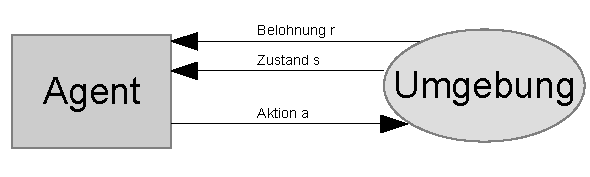
\includegraphics[scale = 1.4]{inhalt/abbildungen/agent_umgebung.pdf}
  \caption{Der Agent und seine Wechselwirkung mit der Umgebung}
  \label{fig:agent_umgebung}
\end{figure} 

Verstärkendes oder auch bestärkendes Lernen beschäftigt sich mit dem Problem, dass ein entscheidungstreffender Agent innerhalb einer unbekannten Umgebung Aktionen (Entscheidungen) ausführen soll (siehe Abbildung \ref{fig:agent_umgebung} \cite[\acs{vgl.} 398]{Alpaydin} und \cite[\acs{vgl.} 290]{Ertel}). Der Agent lernt dann, durch Belohnung oder Bestrafung, seine Aktionen, hinsichtlich seiner Zielstellung, an die Zustände der Umgebung anzupassen. Die Belohnung oder Bestrafung erfolgt jedoch meistens erst nach einer Sequenz von Aktionen, daher ist dem Agenten nicht bekannt ob eine einzelne Aktion positiv oder negativ, hinsichtlich der Erreichung seiner Ziele, ist. Die Optimierung einer solchen Aktionssequenz ist besonders schwierig und daher ein bedeutsames Problem des verstärkenden Lernens.\\

\myparagraph{Ein Agent im Labyrinth}
Nehmen wir an es existiere folgender Agent. Dieser Agent kann vier Aktionen ausführen, bewege dich nach oben, unten, rechts oder links. Er wird in einem ihm unbekannten Labyrinth ausgesetzt. Das Labyrinth ist die Umgebung und die Zustände der Umgebung verändern sich durch die Aktionen des Agenten, das heißt verändert der Agent seine Position innerhalb des Labyrinths, dann wechselt er von einem Ausgangszustand, durch eine Aktion, in einen neuen Zustand der Umgebung. \\

Der Agent lernt also, dass die Aktion 'bewege dich nach oben' den Ausgangszustand in einen neuen Zustand transformiert. Führt der Agent die Aktion 'bewege dich nach oben' aus, dann ist jedoch die Zustandsveränderung abhängig von der individuellen Umgebung in der sich der Agent befindet. In einem Labyrinth kann der Agent nicht immer alle seiner vier Aktionen ausführen, denn er ist umringt von Mauer die seinen Aktionsradius beschränken. Würde er trotzdem eine unzulässige Aktion ausführen, dann verändert sich der Zustand der Umgebung nicht, denn der Agent würde sprichwörtlich gegen die Wand fahren. Das bedeutet für den Agenten, dass er genau differenzieren muss in welchem Zustand er welche Aktion durchführt und wie er sein Ziel erreichen kann. Das Ziel des Agenten, in diesem Beispiel, ist das erreichen des Labyrinth Ausgangs. \\

Nach einer endlichen Sequenz von Aktionen gelingt es dem Agenten den Ausgang des Labyrinths zu erreichen und er erhält eine nummerische Belohnung für die Zielerreichung. Der Weg, sprich die Sequenz von Aktionen, den der Agent, durch probieren und scheitern, gewählt hat wird nicht der schnellstmögliche Weg sein und auch nicht der kürzeste. Wie kann dies Aktionssequenz hinsichtlich der Zielerreichung optimiert werden? \\

\subsection{Die optimale Strategie}
Der Zustand $s_t \in S$ beschreibt die Position eines Agenten in einer Umgebung zu einem festgelegten Zeitpunkt t. S ist eine menge von möglichen Zuständen. Die Aktion $a_t \in A$ wird vom Agenten, zum Zeitpunkt t, ausgeführt und verändert die Umgebung(siehe Abbildung \ref{fig:agent_umgebung}). Diese Aktion überführt den vorherigen Zustand $s_t$ in einen neuen zustand $s_t+1$. Der neue Zustand $s_t+1 = \delta(s_t, a_t)$ wird von der Übergangsfunktion $\delta$ bestimmt. Die Übergangsfunktion wird von der Umgebung bestimmt und kann von dem Agenten nicht beeinflusst werden. Führt ein Agent eine Aktion a in einem Zustand s zu einem Zeitpunkt t aus, dann erhält der Agent eine direkte Belohnung(engl. immediate reward) $t_t = r(s_t, a_t)$. Diese direkte Belohnung ist abhängig von dem aktuellen Zustand und der ausgeführten Aktion.\\

Viele praktische Probleme hingegen haben für jede Aktion in jedem Zustand keine direkte Belohnung. Bei einem Schachspiel zum Beispiel erhält der Agent erst eine positive Belohnung, wenn das Spiel gewonnen ist oder eine negative Belohnung, wenn das Spiel verloren ist. Die zahlreichen vorherigen Aktionen des Agenten erhalten kein Feedback oder eine direkte Belohnung von $r_t(s_t, a_t) = 0$. Eine Schwierigkeit ist diese verspätete Belohnung am Ende einer Aktionssequenz auf die einzelnen Aktionen des Agenten aufzuteilen(engl. credit assignment problem).

\cite[290]{Ertel}   

\subsection{Zeitliche Beschränkung}
Endliches Horizont Modell mit h Schritten

Hat der Agent nur eine endliche Anzahl von Schritten h zur Verfügung, dann ist sein Aktionsradius beschränkt d.h. sein Verhalten verändert sich hinsichtlich der Anzahl der Schritte die dem Agenten zur Verfügung stehen. 

\begin{equation}
E(\sum_{t=0}^{h} r_t)
\end{equation}


Unendliches Horizont Modell
\begin{equation}
E(\sum_{t=0}^{\infty} \gamma^t r_t)
\end{equation}

\subsection{Überwachtes \acs{vs.} verstärkendes Lernen}
Im Gegensatz zu den Lernverfahren beim überwachten Lernen fehlt dem Agenten beim verstärkenden Lernen ein Lehrer der dem Agenten genau sagt ob seine Aktion richtig oder falsch ist. Zudem wäre ein Lehrer, der dem Agenten für jeden Zustand genau sagt welches die richtige Aktion ist, sehr kostspielig. Oftmals ist für einen Zustand gar keine optimale Aktion möglich, erst die Aneinanderreihung von Aktionen und Zustandsübergängen kann optimal sein oder optimiert werden\cite[\acs{vgl.} 397]{Alpaydin}. \\

Ein überwachtes Lernverfahren wird zuerst mittels eines Trainingssets kontrolliert belehrt. Das Trainingsset für ein überwachtes Lernverfahren besteht aus verschiedenen Eigenschaften (Features) und einer den Eigenschaften zugeordneten Klasse beziehungsweise Zielvariable (Target Variable). Die Qualität der Zielwerte kann mittels Testsets ermittelt werden. Ein Testset ist ein Datenset bestehend aus Eigenschaften ohne die dazugehörigen Klassen. Abbildung \ref{fig:vogel_spezies} zeigt, wie ein Trainingsset aussehen könnte\cite[8]{Harrington}. Die Spalten Gewicht, Flügelspanne, Schwimmhäute und Rückenfarbe sind die Eigenschaften und die Spalte Spezies beinhaltet die Zielvariablen. Das überwachte Lernverfahren lernt mittels des Trainingsdatensets die Beziehungen zwischen den Eigenschaften und der Klassen. \\

\begin{figure}[!htbp]
  \centering
  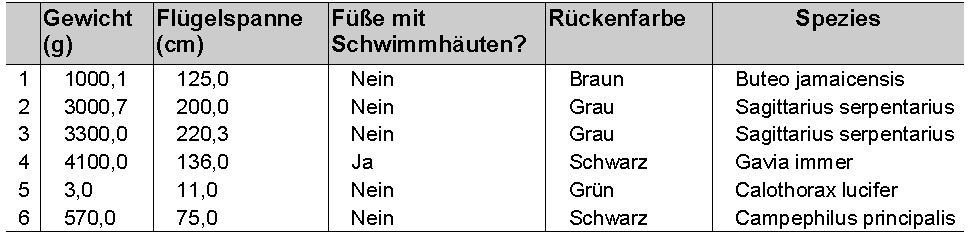
\includegraphics[scale = 0.89]{inhalt/abbildungen/vogel_spezies.pdf}
  \caption{Vogelspezies Klassifikation basierend auf vier Eigenschaften}
  \label{fig:vogel_spezies}
\end{figure} 

Verstärktes Lernen umfasst die Probleme, bei denen in der Regel kein solches Trainingsdatenset vorliegt, welches genau festlegt ob eine Aktion in einem Zustand korrekt oder falsch ist. Bezogen auf ein Testdatenset wäre eine Aktion des Agenten, dass nennen einer Klasse hinsichtlich der gelernten Zusammenhänge aus den Trainingsdaten. Teilt man die Anzahl der korrekten Vorschläge durch die Anzahl aller Versuche, dann erhält man eine Kennzahl für die Qualität der Vorhersage. Sind alle Klassen der Testinstanzen richtig vorhergesagt, dann ist die Kennzahl genau Eins. Jede Zeile eines Testsets und jede Zeile eines Trainingssets ohne die Zielvariablen ist eine Instanz. Verstärkendes Lernen kann trotzdem vom überwachten Lernen profitieren, denn es ist möglich den Agenten in der Anfangsphase des verstärkten Lernens explizit zu programmieren und ihn dadurch auf bestimmte Auffälligkeiten oder Muster aufmerksam zu machen. Ist es zu kompliziert dies explizit zu programmieren, dann kann auch ein Mensch dem Agenten die richtigen Aktionen vorgeben. \\

Sehr nützlich werden diese beiden Unterstützungen der Anfangsphase des verstärkenden Lernens, sobald die Dimensionen der Umwelt oder des Agenten eine bestimmte Größe überschreiten. Eine Aktionsdimension kann sehr wenige Aktionen beinhalten zum Beispiel die vier Aktionen bewege dich nach oben, unten, rechts oder links. Roboter die dem Menschen nachempfunden sind verfügen über bis zu 50 verschiedene Motoren für die einzelnen Gelenke. Diese müssen gleichzeitig angesteuert werden, was zu einem 50-dimensionalen Zustandsraum und einem 50-dimensionalen Aktionenraum führt\cite[\acs{vgl.} 305\psq]{Ertel}. Bei solch großen Dimensionen können die Laufzeiten einiger verstärkender Lernverfahren massiv ansteigen, bis sie praktisch nicht mehr anwendbar sind. Gerade in der Anfangsphase des verstärkten Lernens kann darum ein Eingriff mittels überwachtem Lernen sehr Laufzeit schonend sein.

\subsection{Das Strategiespiel Schach}
Das Strategiespiel Schach hat viele Ähnlichkeiten mit dem Strategiespiel Reversi und auch Ähnlichkeiten zum Spiel Tic Tac Toe, darum wird nachfolgend die  Anwendungsmöglichkeit des verstärkenden Lernens auf das Schachspiel ausführlicher behandelt. \\

\myparagraph{Schachspiel Komplexität}
Während eines Schachspiels gibt es für eine typische Stellung über 30 mögliche Züge und eine durchschnittliche Dauer von 50 Halbzügen ist noch relativ kurz. Würden wir einen Suchbaum \todo{Suchbaum?} für ein Schachspiel aufstellen wollen, dann hätte dieser Suchbaum

\begin{equation}
\sum_{d=0}^{50} 30^{d} = \frac{1 - 30^{51}}{1 - 30} = 7,4 \times 10^{73}
\end{equation}

Blattkonten. Angenommen wir hätten 10.000 Computer, von denen jeder eine Milliarde Schlussfolgerungen pro Sekunde schaffen würde und wir könnten die Arbeit ohne Verlust auf alle Rechner verteilen. Die gesamte Rechenzeit für $7,4 \times 10^{73}$ Schlussfolgerungen wäre dann $\approx 2,3 \times 10^{53}$ Jahre, was wiederum etwa $10^{43}$ mal so lange dauert wie unser Universum alt ist\cite[93 \psq]{Ertel}. \\

Schach ist also äußert komplex und die Dimensionen der Aktions- und Zustandsräume sind sehr groß. Diverse Suchalgorithmen würden an dieser Komplexität scheitern, weil die Rechenzeit dieser Algorithmen exponentiell zu den Dimensionen ansteigt. 

\section{Spielentwicklung}

\section{Lineare Algebra}

\section{Heuristik}